\section{Limitations of Current Practice in Multi-Streamed SSDs}
In this section, we review the key weaknesses of existing stream management techniques 
as well as stream implementation methods.  
\textsf{\small PCStream} was motivated to overcome these weaknesses so that multi-streamed
SSDs can be widely employed in practice.

\begin{figure*}[t]
	\minipage{0.63\textwidth}
	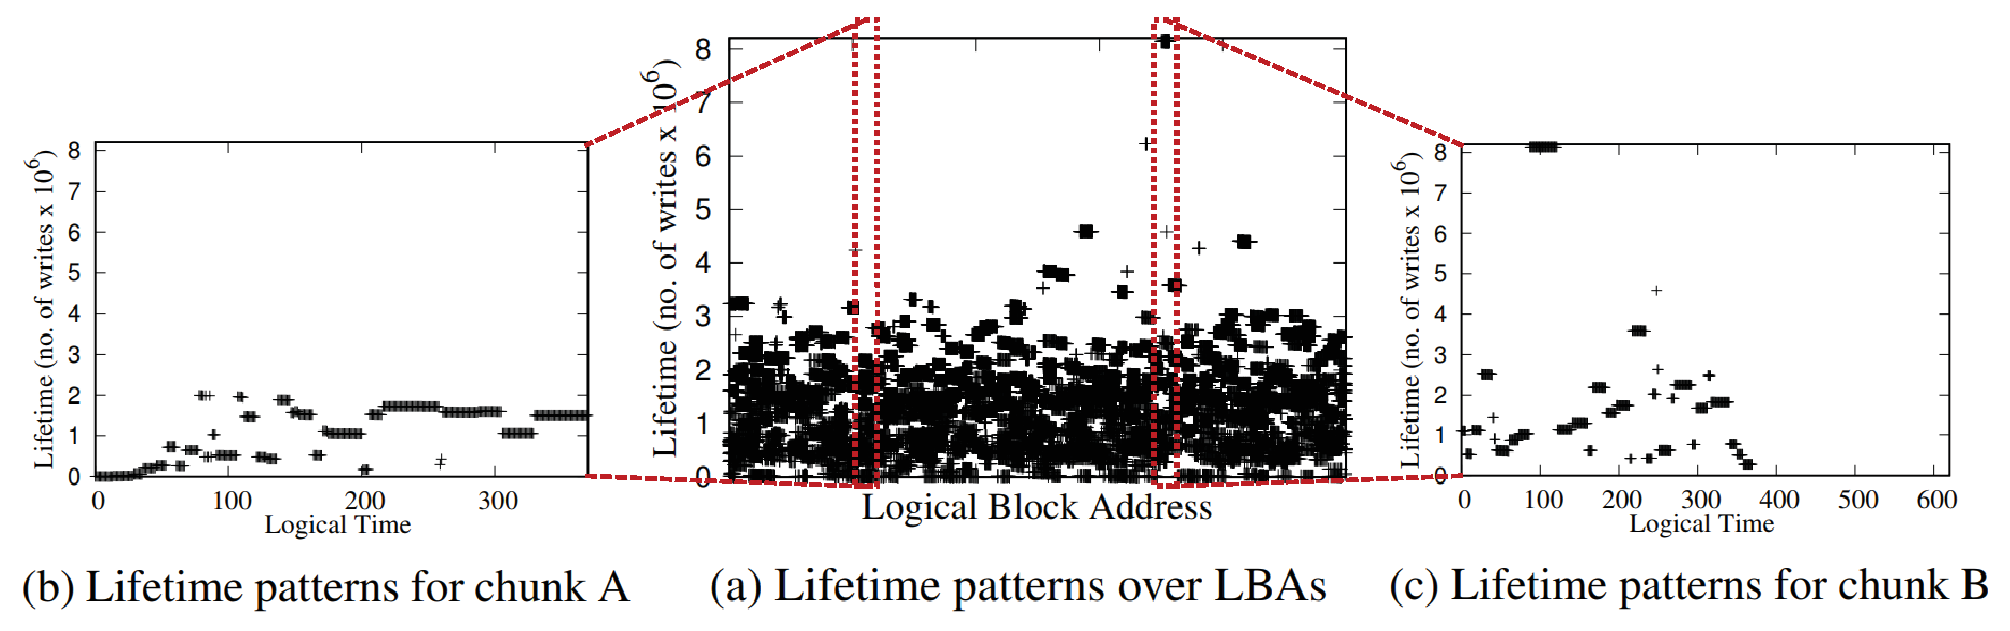
\includegraphics[width=\linewidth]{figure/fig1}
	\caption{Lifetime distributions of append-only workload over addresses and times.}
	\label{fig:lba_lifetime}
	\endminipage \hfill
	\minipage{0.32\textwidth}
	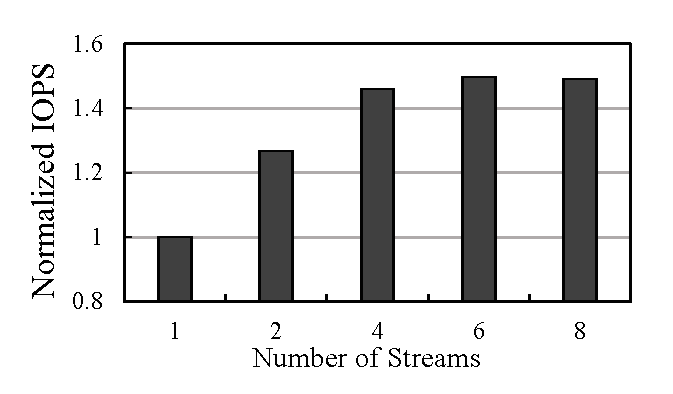
\includegraphics[width=\linewidth]{figure/stream_perf}
	%\caption{Changes in IOPS over varying number of streams.}
	%\caption{IOPS with varying streams.}
	\caption{IOPS changes over the number of streams.}
	\vspace{-20pt}
	\label{fig:stream_perf}
	\endminipage 
\end{figure*}


\subsection{No Automatic Stream Management for General I/O Workloads}
%\subsection{\note{No Automatic Stream Management}}
Most existing stream management techniques~\cite{MultiStream, Level, vStream} 
require programmers to manually allocate streams for their applications.
For example, 
in both \textsf{\small ManualStream\footnote{For brevity, we denote the manual stream allocation
method used in ~\cite{MultiStream} by \textsf{\scriptsize ManualStream}.}}~\cite{MultiStream} and 
~\cite{Level}, there is no systematic guildeline on how to
allocate streams for a given application. 
The efficiency of stream allocations largely depends on the programmer's 
understanding and expertise on data temperature ({\it i.e.}, frequency of updates)
and internals of database systems.
Furthermore, many
techniques also assume that the number of streams is known {\it a priori}.  
Therefore, when an SSD with a different number of streams is used, 
these techniques need to re-allocate streams manually.
\textsf{\small vStream}~\cite{vStream} 
is an exception to this 
restriction by allocating streams to virtual streams, not external streams.  
However, even in \textsf{\small vStream}, virtual stream allocations are left to
programmer's decisions.

\begin{comment}
\begin{figure}[t]
	\centering
	%\vspace{-9pt}
	%\captionsetup[subfigure]{margin={0cm,1cm}}
	\subfloat[Lifetime patterns over LBAs]{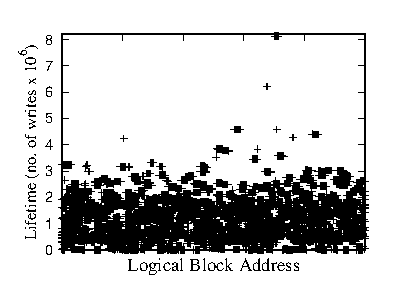
\includegraphics[width=0.25\textwidth]{figure/lifetime_lba_new.eps}}  % data from 0/03031641
	%\subfloat[Lifetime patterns over LBAs for update workload]{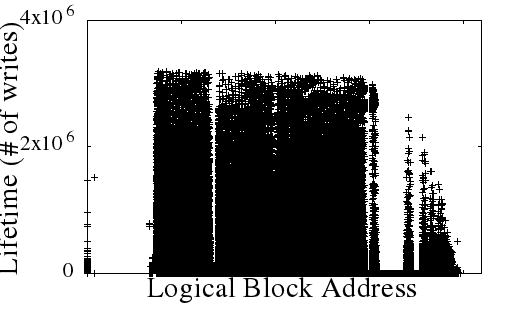
\includegraphics[width=0.215\textwidth]{figure/update_lifetime}}  

	\hfill

	\vspace{-10pt}
	\subfloat[Lifetime patterns for chunk A]{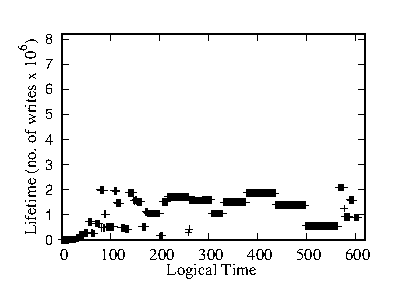
\includegraphics[width=0.21\textwidth]{figure/lifetime_in_chunk1_new.eps}} % data from 0/03031641
	\hspace{10pt}
	\subfloat[Lifetime patterns for chunk B]{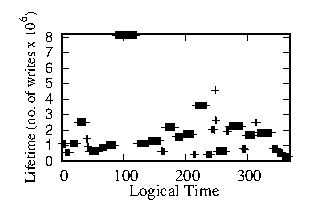
\includegraphics[width=0.21\textwidth]{figure/lifetime_in_chunk4_new.eps}}
	%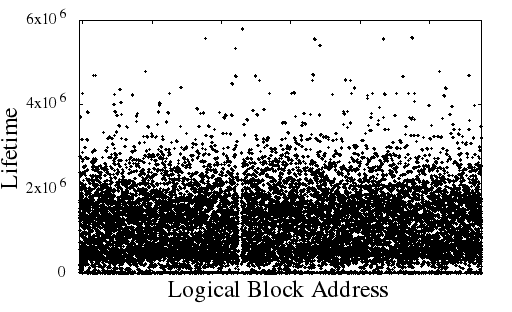
\includegraphics[width=0.9\linewidth]{figure/lba_lifetime} 
	\vspace{-3pt}
	\caption{Lifetime distributions of append-only workload over addresses and times.} %shane part
	\label{fig:lba_lifetime}
	\vspace{-20pt}
\end{figure}
\end{comment}

Although \textsf{\small FStream}~\cite{FStream} and \textsf{\small AutoStream}~\cite{AutoStream}
may be considered 
as automatic stream management techniques,
their applicability is quite limited.
\textsf{\small FStream}~\cite{FStream} can be useful for separating file system metadata but it does not
work for the user data separation.
\textsf{\small AutoStream}~\cite{AutoStream} is the only known technique that works in a 
fully automatic fashion by making stream allocation decisions within 
the kernel.
However, since \textsf{\small AutoStream} predicts data lifetimes using the
access frequency of the same LBA, \textsf{\small AutoStream} does not work well 
when no apparent {\it locality} on LBA accesses exists in applications.  
For example, in recent data-intensive applications 
such as RocksDB~\cite{RocksDB} and Cassandra~\cite{Cassandra}, 
majority of data are written in an append-only manner,
thus no LBA-level locality can be detected inside an SSD.

In order to illustrate a mismatch between an LBA-based data separation technique and 
append-only workloads, we analyzed the write pattern of 
RocksDB~\cite{RocksDB}, which is a
popular key-value store based on the LSM-tree algorithm~\cite{LSM}.
Fig.~\ref{fig:lba_lifetime}(a) shows how LBAs may be related 
to data lifetimes in RocksDB.  
We define the lifetime of data as the interval length (in terms of
the logical time based on the number of writes) between
when the data is first written and when the data is invalidated
by an overwrite or a TRIM command~\cite{TRIM}.
As shown in Fig.~\ref{fig:lba_lifetime}(a), 
there is no strong correlation between LBAs and their lifetimes in RocksDB.  

We also analyzed 
if the lifetimes of LBAs change under some predictable patterns over time 
although the overall lifetime distribution shows large variances.
Figs.~\ref{fig:lba_lifetime}(b) and~\ref{fig:lba_lifetime}(c) show
scatter plots of data lifetimes over the logical time 
for two specific 1-MB chunks with 256 pages. 
As shown in Figs.~\ref{fig:lba_lifetime}(b) and~\ref{fig:lba_lifetime}(c), 
for the given chunk, the lifetime of data written to the chunk 
varies in an unpredictable fashion.  
For example, at the logical time 10 in Fig.~\ref{fig:lba_lifetime}(b), 
the lifetime was 1 but it increases about 
2 million around the logical time 450 
followed by a rapid drop around the logical time 500. 
Our workload analysis using RocksDB strongly suggests that under append-only workloads, 
LBAs are not useful in predicting data lifetimes reliably.
In practice, the applicability of LBA-based data separation techniques is quite 
limited to a few cases only when the LBA access
locality is obvious in I/O activities such as updating metadata files or log files.  
In order to support {\it general} I/O workloads in an automatic fashion, stream 
management decisions should be based on higher-level information
which do not depend on lower-level details such as write patterns based on LBAs.

\begin{comment}
\begin{figure}[t]
	\centering
	%\vspace{-10pt}
	%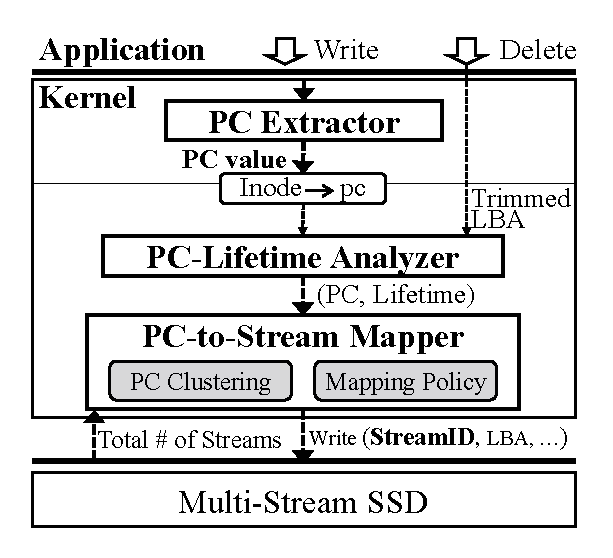
\includegraphics[width=0.6\linewidth]{figure/architecture4}
	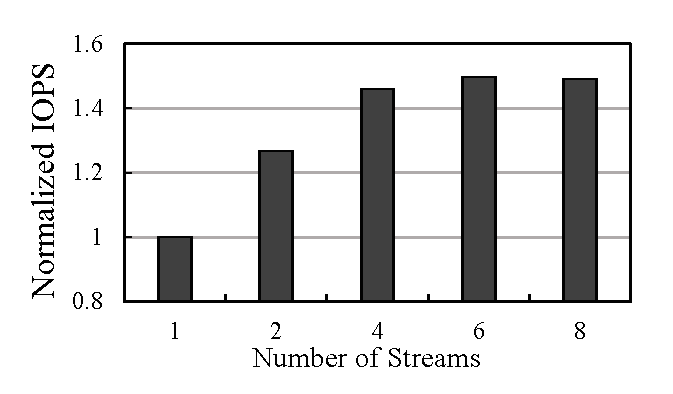
\includegraphics[width=0.7\linewidth]{figure/stream_perf}
	\vspace{-9pt}
	\caption{Changes in IOPS over varying number of streams.} 
	\label{fig:stream_perf}
	\vspace{-15pt}
\end{figure}
\end{comment}

\subsection{Limited Number of Supported Streams}
One of the key performance parameters in multi-streamed SSDs is the number of
available streams in SSDs.  Since the main function of  streams is to separate
data with different lifetimes so that they are not mixed in the same block, it
is clear that the higher the number of streams, the more efficient the
performance of multi-streamed SSDs.  For example, Fig.~\ref{fig:stream_perf}
shows how IOPS in RocksDB changes as the number of streams increases on a
Samsung PM963 multi-streamed SSD with 9 streams.  The \texttt{db\_bench}
benchmark was used for measuring IOPS values with streams manually allocated.
As shown in Fig.~\ref{fig:stream_perf}, the IOPS is continuously improving
until 6 streams are used when dominant I/O activities with different data
lifetimes are sufficiently separated.  In order to support a large number of
streams, both the SBC-4 and NVMe revision 1.3, which define the multi-stream
related specifications, allow up to 65,536 streams~\cite{T10, NVMe}.  However,
the number of streams supported in commercial SSDs is quite limited, say, 4 to
16~\cite{MultiStream, Level, AutoStream}, because of several implementation
constraints on the backup power capacity and fast memory size.

These constraints are directly related to a write buffering mechanism that is
commonly used in modern SSDs.   In order to improve the write throughput while
effectively hiding the size difference between the FTL mapping unit and the
flash program unit, host writes are first buffered before they are written to
flash pages in a highly parallel fashion for high performance.  Buffering host
writes temporarily inside SSDs, however, presents a serious data integrity risk
for storage systems when a sudden power failure occurs.  In order to avoid such
critical failures, in data centers or storage servers where multi-streamed SSDs
are used, SSDs use tantalum or electrolytic capacitors as a backup power
source.  When a main power is suddenly failed, the backup power is used to
write back the buffered data reliably.  Since the capacity of backup power is
limited because of the limited PCB size and its cost, the maximum amount of
buffered data is also limited.  In multi-streamed SSDs where each stream needs
its own buffered area, the amount of buffered data increases as the number of
streams increases.  The practical limit in the capacity of backup power,
therefore, dictates the maximum number of streams as well.

The limited size of fast memory, such as TCM~\cite{TCM} or SRAM, is another
main hurdle in increasing the number of streams in multi-streamed SSDs.  Since
multi-stream related metadata which includes data structures for write
buffering should be accessed quickly as well as frequently, most SSD
controllers implement data structures for supporting streams on fast memory
over more common DRAM.  Since the buffered data is the most recent one for a
given LBA, each read request needs to check if the read request should be
served from the buffered data or not.  In order to support a quick checkup of
buffered data, probabilistic data structures such as a bloom filter can be used
along with other efficient data structures, for accessing LBA addresses of
buffered data and for locating buffer starting addresses.   Since the latency
of a read request depends on how fast these data structures can be accessed,
most SSDs place the buffering-related data structure on fast memory.
Similarly, in order to quickly store buffered data in flash chips, these data
structure should be placed on fast memory as well.  However, most SSD
manufacturers are quite sensitive in increasing the size of fast memory because
it may increase the overall SSD cost.   A limited size of fast memory,
unfortunately, restricts the number of supported streams quite severely.

